\documentclass{article}
\usepackage{subfiles}
\usepackage{forest}
\usetikzlibrary{shadows,arrows.meta}
\usepackage{float}
\usepackage{colortbl}
%A4 page size = 210mm, 297mm / inset total = size-margin
\usepackage[a4paper, total={190mm, 277mm}]{geometry}
\usepackage{fontspec}
%\setmainfont{TimesNewRoman}

\title{}
\author{}
\begin{document}
\large

\section{Overall Project Plan}
\subsection{Network Diagram}
    \begin{figure}[H]
      \centering
      \begin{tabular}{|p{0.65cm}|p{5cm}|p{3cm}|l|l|} \hline
        \textbf{Task} & \textbf{Description} &
        \textbf{Duration} & \textbf{Float} & \textbf{Slack}
        \\ \hline
        \rowcolor{green!10} A1  & Research requirements    &
        10 days  & 0 & 0 \\ \hline
        \rowcolor{green!15} A2  & Plan business operations &
        8 days  & 0 & 0 \\ \hline
        \rowcolor{green!20} A3  & Acquire Funding    &
        5 days  & 90 & 15 \\ \hline
        \rowcolor{green!25} A4  & Produce Product prototype &
        9 days  & 0 & 0 \\ \hline
        \rowcolor{green!30} A5  & Test prototype for Quality &
        3 days  & 0 & 0 \\ \hline
        \rowcolor{green!35} A6  & Acquire Material sourcing contracts &
        3 days  & 78 & 0 \\ \hline
        \rowcolor{green!40} A7  & Acquire Transport contracts &
        2 days  & 77 & 10 \\ \hline
        \rowcolor{blue!10} A8  & Acquire marketing contracts &
        4 days  & 79 & 0 \\ \hline
        \rowcolor{blue!15} A9  & Equipment supplier contracts &
        3 days & 78 & 0 \\ \hline
        \rowcolor{blue!20} A10 & Setup storage room and inventory system &
        7 days  & 75 & 5 \\ \hline
        \rowcolor{blue!25} A11 & Setup factory &
        27 days & 82 & 0 \\ \hline
        \rowcolor{blue!30} A12 & Receive and install equipment &
        9 days  & 82 & 0 \\ \hline
        \rowcolor{blue!35} A13 & Receive Material &
        1 day & 80 & 35 \\ \hline
        \rowcolor{blue!40} A14 & Produce produt batch &
        6 days  & 82 & 0 \\ \hline
        \rowcolor{red!10}  A15 & Create social media presence and adverts &
        2 days  & 79 & 2 \\ \hline
        \rowcolor{red!15} A16 & Create company website &
        4 days  & 79 & 0 \\ \hline
        \rowcolor{red!20} A17 & Run traditional advertisements that link back to website and
        social media &
        Run Until first batch ships (47 days)  & 69 & 0 \\ \hline
        \rowcolor{red!25} A18 & Ship product batch to dealers &
        10 days  & 82 & 0 \\ \hline
        \rowcolor{red!30} A19 & Collect and analyse buyer habits, marketing and product performance metrics &
        28 days & 82 & 0 \\ \hline
        \rowcolor{red!35} A20 & Implement improvements based on collected information &
        13 days  & 82 & 0 \\ \hline
      \end{tabular}
    \end{figure}


    \tikzset{
      every node/.style={},
      style1/.style= {draw,text width=1cm,rectangle,align=center},
      stylecp/.style= {thick,draw=red!256},
    }
    \begin{figure}[H]
      \scriptsize
      \begin{tikzpicture}[
        node distance=1.5cm,
        ]
        \newcommand{\tab}{\ \ \ \ };  
        \node[style1,fill=green!10]                (A1)  {0 \tab 10 \\ A1  \\ 10 \\ 0 \tab 10};
        \node[style1,fill=green!15,right of = A1]  (A2)  {10 \tab 18 \\ A2 \\ 8 \\ 10 \tab 18};
        \node[style1,fill=green!20,below of = A2]  (A3)  {10 \tab 15 \\ A3 \\ 5  \\ 100 105};
        \node[style1,fill=green!25,right of = A2]  (A4)  {18 \tab 27 \\ A4  \\ 9  \\ 18 \tab 27};
        \node[style1,fill=green!30,right of = A4]  (A5)  {17 \tab 30 \\ A5  \\ 3  \\ 17 \tab 30};
        \node[right of = A5]  (S50) {};

        \node[style1,fill=blue!15,right of = S50] (A9)  {30 \tab 33 \\ A9  \\ 3 \\ 108 111};
        \node[style1,fill=green!40,above of = A9]  (A7)  {30 \tab 32 \\ A7  \\ 2 \\ 107 109};
        \node[style1,fill=blue!30,right of = A9]  (A12) {33 \tab 42 \\ A12 \\ 9 \\ 115 124};
        
        \node[style1,fill=blue!25,right of = A12] (A11) {42 \tab 69 \\ A11 \\ 27 \\ 124 151};
        \node[right of = A11] (S110){};
        \node[right of = S110](S111){};

        \node[style1,fill=red!30,right of = S111](A19) {85 \ 113 \\ A19 \\ 28 \\ 167 195};
        \node[style1,fill=red!35,right of = A19] (A20) {113 126 \\ A20 \\ 13 \\ 195 208};

        \node[style1,fill=green!35,above of = A7]  (A6)  {30 \tab 33 \\ A6  \\ 3 \\ 108 111};
        \node[style1,fill=blue!35,right of = A6]  (A13) {33 \tab 34 \\ A13 \\ 1 \\ 113 114};

        \node[style1,fill=blue!20,below of = A9]  (A10) {30 \tab 37 \\ A10 \\ 7 \\ 105 112};
        \node[style1,fill=blue!10,below of = A10] (A8)  {30 \tab 34 \\ A8  \\ 4 \\ 109 113};
        \node[style1,fill=red!10,right of = A8]  (A15) {34 \tab 36 \\ A15 \\ 2 \\ 113 115};
        \node[style1,fill=red!15,below of = A15] (A16) {34 \tab 38 \\ A16 \\ 4 \\ 113 117};
        \node[style1,fill=red!20,right of = A15] (A17) {38 \tab 85 \\ A17 \\ 47 \\ 117 154};
        \node[right of = A17](S150){};
        \node[right of = S150](S151){};

        \node[right of = A7]  (S70) {};
        \node[right of = S70] (S71) {};
        \node[style1,fill=blue!40,right of = S71] (A14) {69 \tab 75 \\ A14 \\ 6 \\ 151 157};
        \node[style1,fill=red!25,right of = A14] (A18) {75 \tab 85 \\ A18 \\ 10 \\ 157 167};

        \draw[->] (A1.east) -- (A2.west);
        \draw[->] (A2.east) -- (A4.west);
        \draw[->] (A4.east) -- (A5.west);
        \draw[->] (A5.east) -- (A9.west);
        \draw[->] (A9.east) -- (A12.west);
        \draw[->] (A12.east) -- (A11.west);
        \draw[->] (A6.east) -- (A13.west);
        \draw[->] (A8.east) -- (A15.west);
        \draw[->] (A15.east) -- (A17.west);
        \draw[->] (A14.east) -- (A18.west);
        \draw[->] (A19.east) -- (A20.west);


        \draw (0.70cm,0cm) -- (0.7cm,-1.5cm);
        \draw[->] (0.70cm,-1.5cm) -- (A3.west);
        \draw (A3.east) -- (5.2cm,-1.5cm);

        \draw (5.2cm,0cm) -- (5.2cm,-1.5cm);

        \draw (6.6cm,3cm) -- (6.6cm,-3cm);
        \draw[->] (6.6cm,3cm) -- (A6.west);
        \draw[->] (6.6cm,1.5cm) -- (A7.west);
        \draw[->] (6.6cm,-1.5cm) -- (A10.west);
        \draw[->] (6.6cm,-3cm) -- (A8.west);

        \draw (9.7cm,1.5cm) -- (9.7cm,-1.5cm);
        \draw (A7.east) -- (9.7cm,1.5cm);
        \draw (A10.east) -- (9.7cm,-1.5cm);

        \draw (11.2cm,3cm) -- (11.2cm,0cm);
        \draw (A13.east) -- (11.2cm,3cm);
        \draw (A11.east) -- (11.2cm,0cm);
        \draw[->] (11.2cm,1.5cm) -- (A14.west);

        \draw (8.2cm,-3cm) -- (8.2cm,-4.5cm);
        \draw[->] (8.2cm,-4.5cm) -- (A16.west);
        \draw (9.7cm,-3cm) -- (9.7cm,-4.5cm);
        \draw (A16.east) -- (9.7cm,-4.5cm);

        \draw (14.2cm,1.5cm) -- (14.2cm,-3cm);
        \draw (A17.east) -- (14.2cm,-3cm);
        \draw (A18.east) -- (14.2cm,1.5cm);
        \draw (14.2cm,0cm) -- (A19.west);

      \end{tikzpicture}
      \caption{Overall Project network diagram}
    \end{figure}

    \subsection{Systems thinking \& Business structure integratedness}
    \begin{figure}[H]
      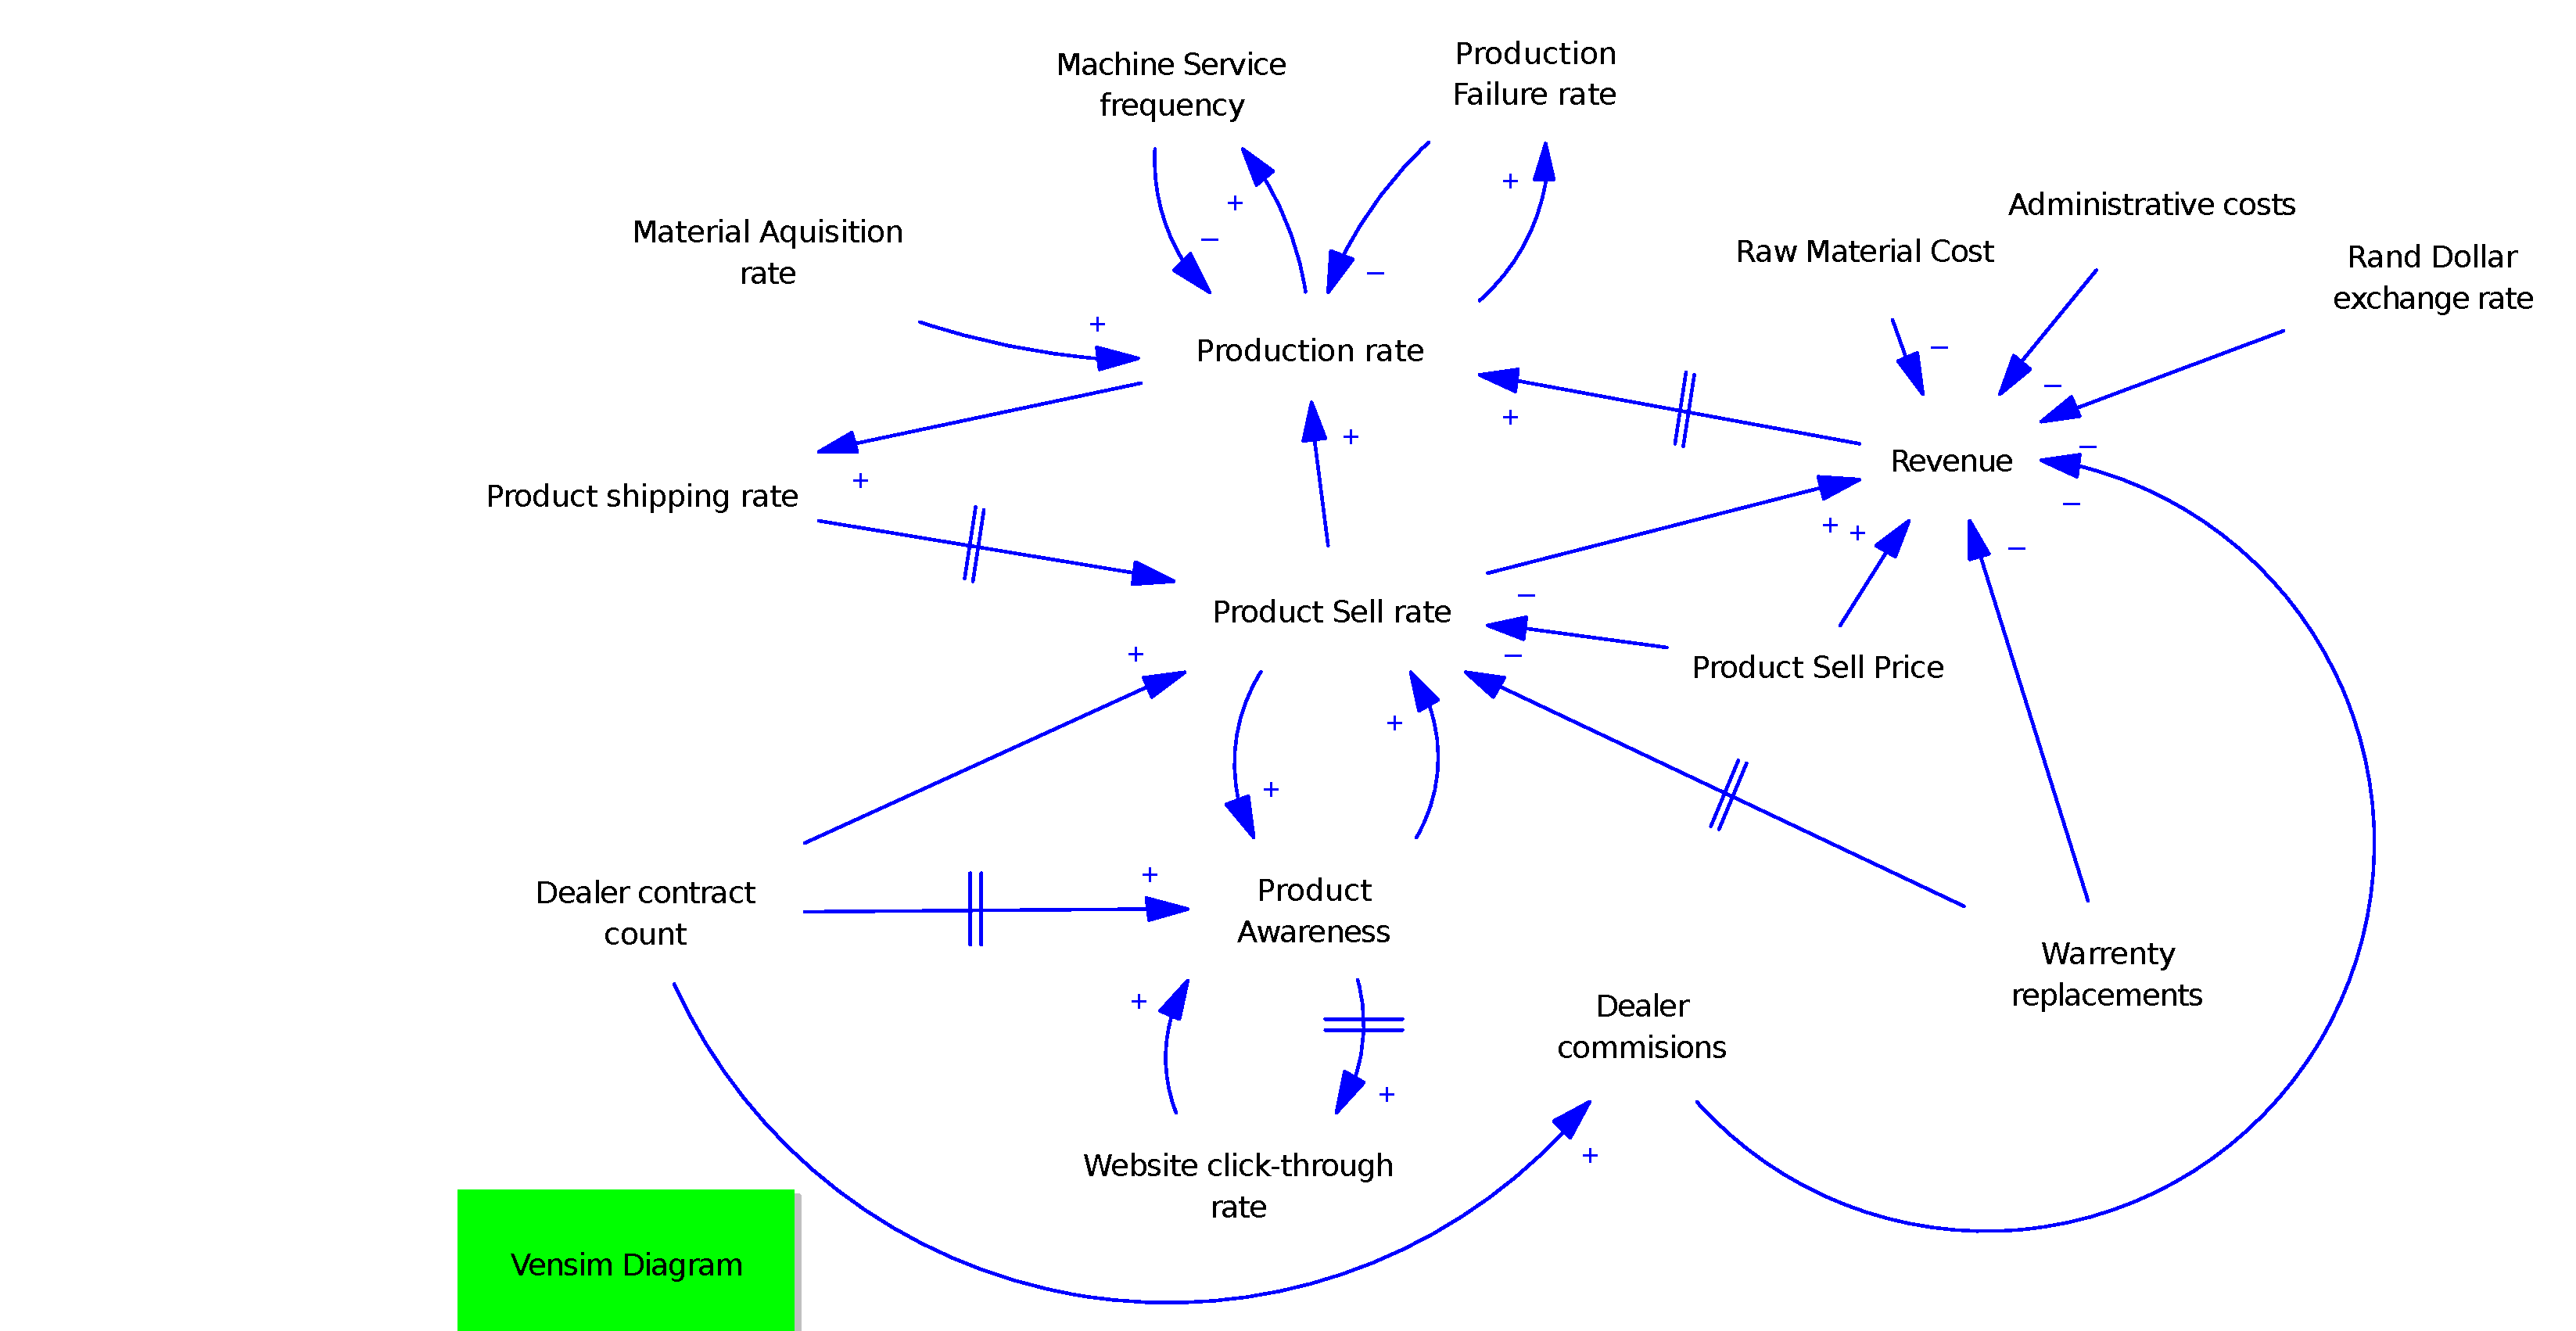
\includegraphics[width=1\linewidth]{figures/Vensim_Diagram.pdf}
      \caption{Vensim business structure diagram}
    \end{figure}
\end{document}
